\begin{problem}{C1}
Sketch a solution curve through each point marked in the slope field.

\begin{center}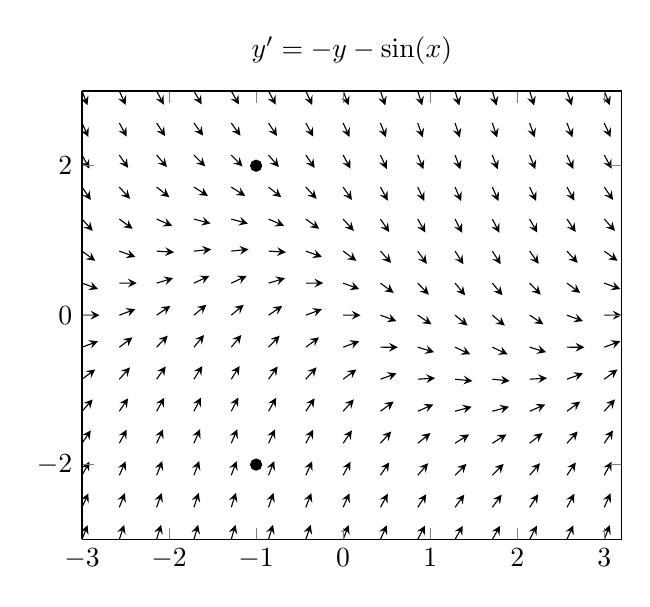
\begin{tikzpicture}
    \begin{axis}[
        title={\(y' = -y - \sin(x)\)},
        domain=-3:3,
        view={0}{90},
        axis background/.style={fill=white},
    ]
        \addplot3[black,
            quiver={
             u={1/(sqrt(1 + (-y - sin(60*x))^2)},
             v={(-y - sin(60*x))/(sqrt(1 + (-y - sin(60*x))^2)},
             scale arrows=0.2,
            },
            -stealth,samples=15]
                {exp(-x) - 1/2*sin(x) - 1/2*cos(x)};
        %KAWWWWWWW
        % Here be some points added to the swoopy loop vector fieldamagigs
        \addplot[mark=*] coordinates {(-1,2)}; % Obvious ordered pair for lococation
        \addplot[mark=*] coordinates {(-1,-2)};
    \end{axis}
\end{tikzpicture}\end{center}
\end{problem}

\begin{problem}{C1}
Sketch a solution curve through each point marked in the slope field.

\begin{center}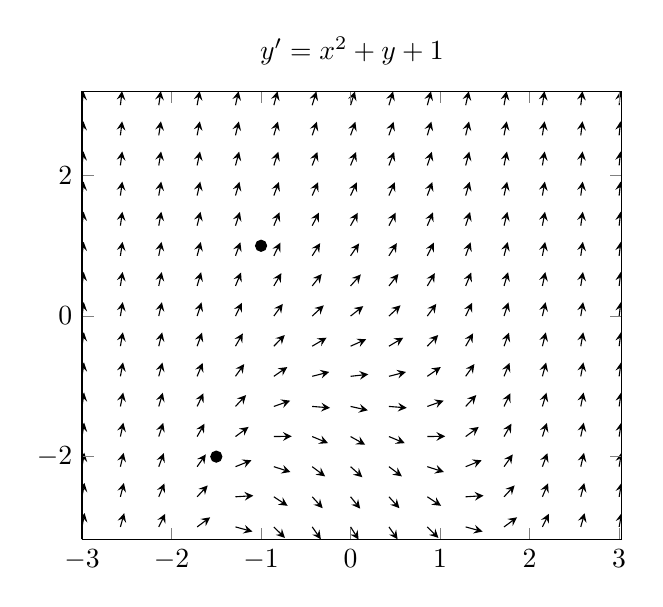
\begin{tikzpicture}
    \begin{axis}[
        title={\(y' = x^2 + y+1\)},
        domain=-3:3,
        view={0}{90},
        axis background/.style={fill=white},
    ]
        \addplot3[black,
            quiver={
             u={1/sqrt(1 + (x^2+y+1)^2)},
             v={(x^2 + y+1)/sqrt(1 + (x^2+y+1)^2)},
             scale arrows=0.2,
            },
            -stealth,samples=15]
                {exp(x) - x - 1};
        %KAWWWWWWW
        % Here be some points added to the swoopy loop vector fieldamagigs
        \addplot[mark=*] coordinates {(-1,1)}; % Obvious ordered pair for lococation
        \addplot[mark=*] coordinates {(-1.5,-2)};
    \end{axis}
\end{tikzpicture}\end{center}
\end{problem}

\begin{problem}{C1}
Sketch a solution curve through each point marked in the slope field.

\begin{center}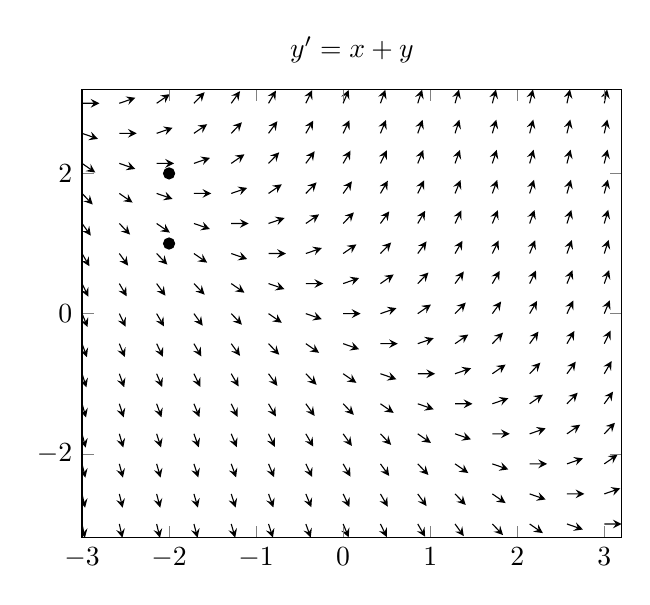
\begin{tikzpicture}
    \begin{axis}[
        title={\(y' = x + y\)},
        domain=-3:3,
        view={0}{90},
        axis background/.style={fill=white},
    ]
        \addplot3[black,
            quiver={
             u={1/sqrt(1 + (x+y)^2)},
             v={(x + y)/sqrt(1 + (x+y)^2)},
             scale arrows=0.2,
            },
            -stealth,samples=15]
                {exp(x) - x - 1};
        %KAWWWWWWW
        % Here be some points added to the swoopy loop vector fieldamagigs
        \addplot[mark=*] coordinates {(-2,1)}; % Obvious ordered pair for lococation
        \addplot[mark=*] coordinates {(-2,2)};
    \end{axis}
\end{tikzpicture}\end{center}
\end{problem}

\begin{problem}{C1}
Sketch a solution curve through each point marked in the slope field.

\begin{center}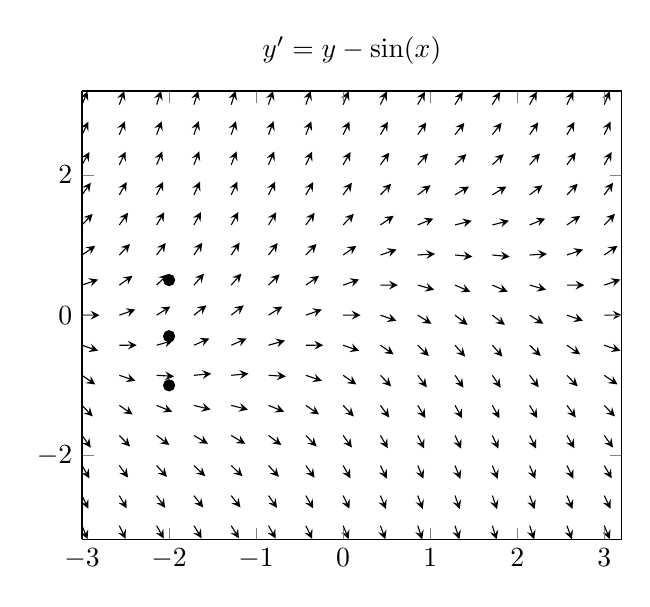
\begin{tikzpicture}
    \begin{axis}[
        title={\(y' = y - \sin(x)\)},
        domain=-3:3,
        view={0}{90},
        axis background/.style={fill=white},
    ]
        \addplot3[black,
            quiver={
             u={1/sqrt(1 + (y-sin(60*x))^2)},
             v={(y - sin(60*x))/sqrt(1 + (y-sin(60*x))^2)},
             scale arrows=0.2,
            },
            -stealth,samples=15]
                {exp(x) + 1/2*sin(x) + 1/2*cos(x)};
        %KAWWWWWWW
        % Here be some points added to the swoopy loop vector fieldamagigs
        \addplot[mark=*] coordinates {(-2,-1)}; % Obvious ordered pair for lococation
        \addplot[mark=*] coordinates {(-2,-.3)};
        \addplot[mark=*] coordinates {(-2,.5)};
    \end{axis}
\end{tikzpicture}\end{center}
\end{problem}

\begin{problem}{C1}
Sketch a solution curve through each point marked in the slope field.

\begin{center}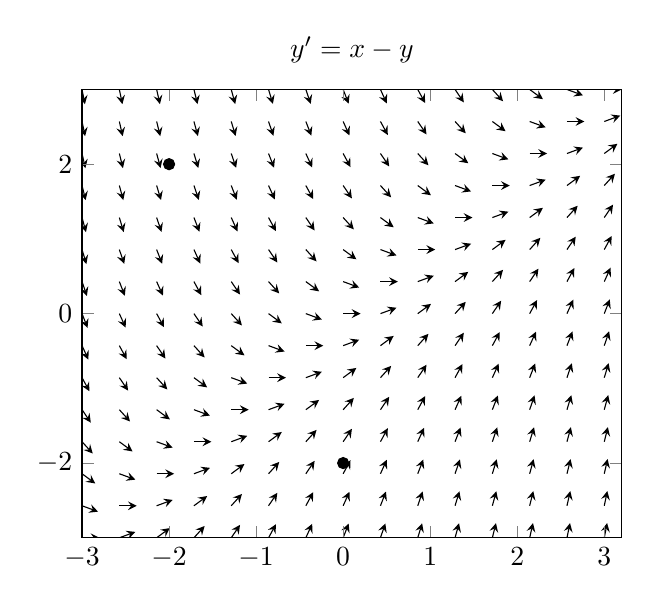
\begin{tikzpicture}
    \begin{axis}[
        title={\(y' = x - y\)},
        domain=-3:3,
        view={0}{90},
        axis background/.style={fill=white},
    ]
        \addplot3[black,
            quiver={
             u={1/sqrt(1 + (x - y)^2)},
             v={(x - y)/sqrt(1 + (x - y)^2)},
             scale arrows=0.2,
            },
            -stealth,samples=15]
                {exp(-x) + x - 1};
        \addplot[mark=*] coordinates {(-2,2)};
        \addplot[mark=*] coordinates {(0,-2)};
    \end{axis}
\end{tikzpicture}\end{center}
\end{problem}

\begin{problem}{C1}
Sketch a solution curve through each point marked in the slope field.

\begin{center}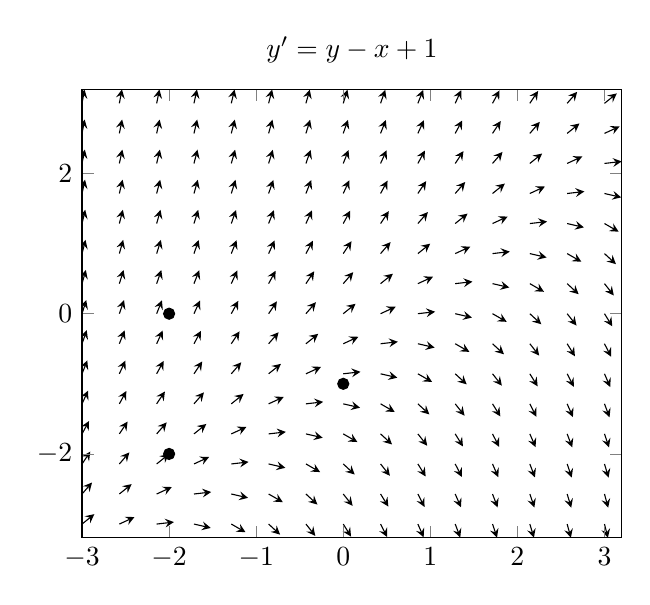
\begin{tikzpicture}
    \begin{axis}[
        title={\(y' = y - x + 1\)},
        domain=-3:3,
        view={0}{90},
        axis background/.style={fill=white},
    ]
        \addplot3[black,
            quiver={
             u={1/sqrt(1 + (y - x + 1)^2)},
             v={(y - x + 1)/sqrt(1 + (y - x + 1)^2)},
             scale arrows=0.2,
            },
            -stealth,samples=15]
                {exp(x) + x};
        \addplot[mark=*] coordinates {(-2,-2)};
        \addplot[mark=*] coordinates {(-2,0)};
        \addplot[mark=*] coordinates {(0,-1)};
    \end{axis}
\end{tikzpicture}\end{center}
\end{problem}

\begin{problem}{C1}
Sketch a solution curve through each point marked in the slope field.

\begin{center}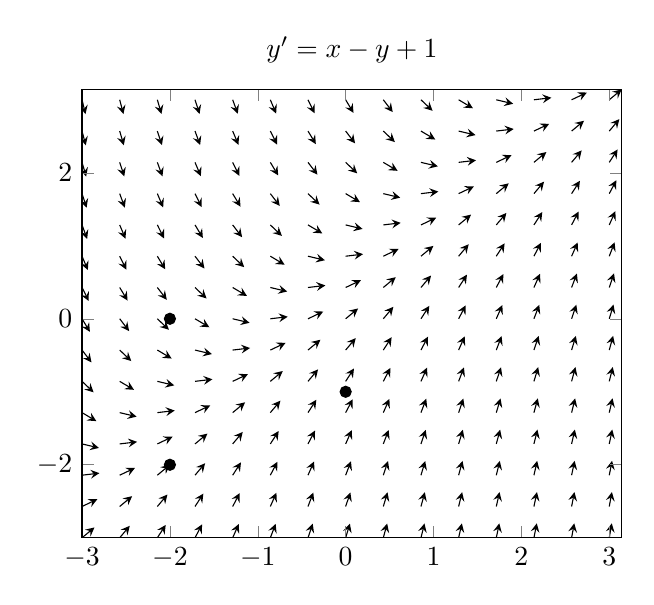
\begin{tikzpicture}
    \begin{axis}[
        title={\(y' = x - y + 1\)},
        domain=-3:3,
        view={0}{90},
        axis background/.style={fill=white},
    ]
        \addplot3[black,
            quiver={
             u={1/sqrt(1 + (x - y + 1)^2)},
             v={(x - y + 1)/sqrt(1 + (x - y + 1)^2)},
             scale arrows=0.2,
            },
            -stealth,samples=15]
                {exp(-x) + x};
        \addplot[mark=*] coordinates {(-2,-2)};
        \addplot[mark=*] coordinates {(-2,0)};
        \addplot[mark=*] coordinates {(0,-1)};
    \end{axis}
\end{tikzpicture}\end{center}
\end{problem}

\begin{problem}{C1}
Sketch a solution curve through each point marked in the slope field.

\begin{center}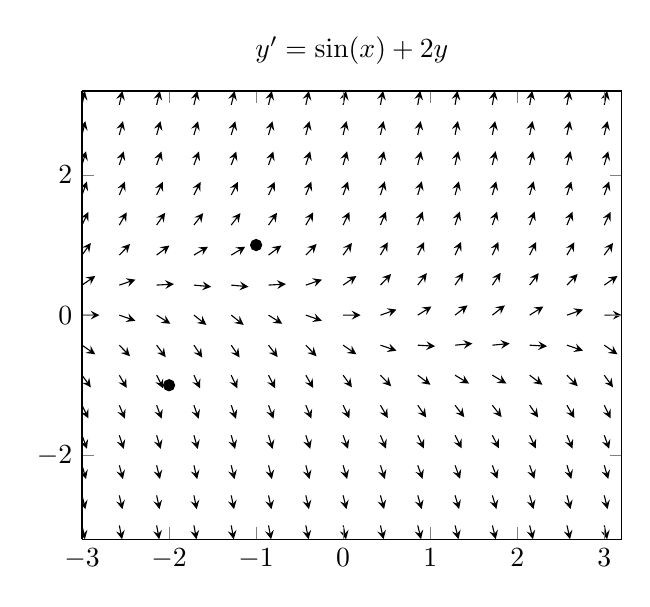
\begin{tikzpicture}
    \begin{axis}[
        title={\(y' = \sin(x) + 2y\)},
        domain=-3:3,
        view={0}{90},
        axis background/.style={fill=white},
    ]
        \addplot3[black,
            quiver={
             u={1/sqrt(1 + (sin(60*x) + 2*y)^2)},
             v={(sin(60*x) +2*y)/sqrt(1 + (sin(60*x) + 2*y)^2)},
             scale arrows=0.2,
            },
            -stealth,samples=15]
                {x};
        \addplot[mark=*] coordinates {(-1,1)};
        \addplot[mark=*] coordinates {(-2,-1)};
    \end{axis}
\end{tikzpicture}\end{center}
\end{problem}

\begin{problem}{C1}
Sketch a solution curve through each point marked in the slope field.

\begin{center}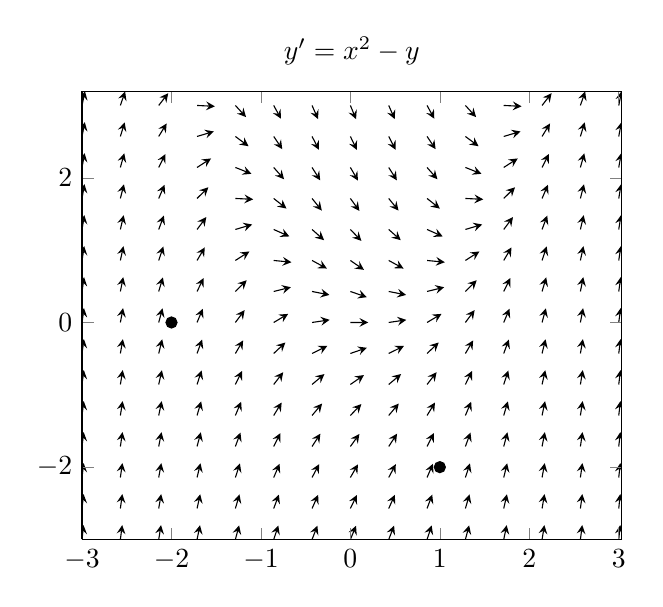
\begin{tikzpicture}
    \begin{axis}[
        title={\(y' = x^2 - y\)},
        domain=-3:3,
        view={0}{90},
        axis background/.style={fill=white},
    ]
        \addplot3[black,
            quiver={
             u={1/sqrt(1 + (x^2 - y)^2)},
             v={(x^2 - y)/sqrt(1 + (x^2 - y)^2)},
             scale arrows=0.2,
            },
            -stealth,samples=15]
                {x};
        \addplot[mark=*] coordinates {(-2,0)};
        \addplot[mark=*] coordinates {(1,-2)};
    \end{axis}
\end{tikzpicture}\end{center}
\end{problem}

